\section{Action Modulation}
The principal role of this sub-system is to convert abstract actions (e.g. walk, gaze, etc.) and the emotional state to actions that could be performed by the robotic platform that it has been using. These emotions actions are just commands to the platform, but the emotional part is added during the process due to adding new simple actions, changing the parameters of the simple actions, or both. This could be done thanks that each abstract action should be describe in terms of simple actions, which the system knows how to modify and perform. The main inputs of these module are:
\begin{itemize}
	\item Emotion profiles, which is the information in how to show an emotion in terms of simple actions.
	\item Action profiles, which describes the basic actions and the composition of the abstract actions in terms of the simple actions. This is not longer truth because getting the information from the file implies that should be possible to generate the code from these files.
	\item Emotional state is described by the tuple emotion and intensity. The first says the emotions that is going to convey the robot, and the second says how much is going to be evident the emotion. Still missing the part of the intensity.
	\item Abstract action, which could be a simple action to a any action described in terms of the simple actions supported by the system.	
	\item Platform descriptions gives the information about which simple actions could be performed by the current platform.
	\item World model.
\end{itemize} 
The outputs of this module are:
\begin{itemize}
	\item \textit{Electronic signals:} to control each driver that has the robot.
	\item \textit{Failure signal:} to inform the action decision sub-system that one of the actions could not be performed.
\end{itemize}
This sub-system is sub-divided into two blocks: actions modulation and action generation.
%%%%%%%%%%%%%%%%%%%%%%%%%
\subsection{Action Modulation}
This module gets the emotional state and the action(s) to generate emotive actions, which includes adding new actions and modifying parameters of the current. To do this module add new actions regarding the platform. The inputs to this module are:
\begin{itemize}
	\item Emotion profiles
	\item Action profiles
	\item Emotional state
	\item Abstract action
\end{itemize}
The outputs:
\begin{itemize}
	\item \textit{Emotional actions:} are the set of simple actions with modified parameters to show emotions.
\end{itemize}
As well this module is divided in modules with specific objectives, the division could be seen in Figure~\ref{fig:actionModulation}. The goal of each module is described below:
\begin{itemize}
	\item \textit{Action decrypt:} take the abstract actions and converted to simple actions.
	\item \textit{Action addition:} add the new actions needed to show the emotion.
	\item \textit{Action modification:} changes the parameters of all the actions.
\end{itemize}
\begin{figure}
	\centering
	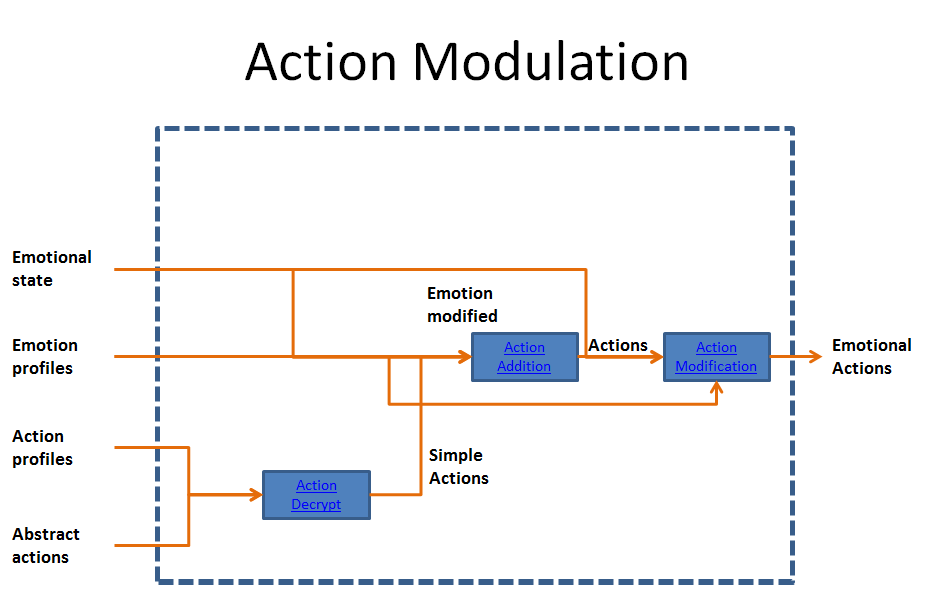
\includegraphics[width=1.0\textwidth]{./Images/Architecture/ActionModulation.png} 
	\caption{Modules of the action modulation sub-system}
	\label{fig:actionModulation}
\end{figure}
%%%%%%%%%%%%%%%%%%%%%%%%%
\subsection{Action Generation}
This module is in charge to decide which actions could be performed by the current platform, and execute and control each action that should be performed. The inputs of this module are:
\begin{itemize}
	\item Platform description
	\item Emotional actions
	\item World model
\end{itemize}
The outputs are:
\begin{itemize}
	\item Failure signal
	\item Signal controls
\end{itemize}
The task decomposition could be seen in Figure~\ref{fig:actionGeneration}. The goal of each sub-module are described below:
\begin{itemize}
	\item \textit{Action filter:} filters the possible actions that could be perform due the constrains of the platform, and it makes any necessary change to the action to be correct performed by the platform (e.g. Constrains of movement)
	\item \textit{Action controller:} decides which actions should be executed given the current actions that have performed by the robot. This module communicates with a specific module, which knows how to perform the action. This module knows which actions are executing and solve the problems of precedence and importance.
	\item \textit{Specific controllers:} are modules developed with the idea to execute an specific simple action.
\end{itemize}
\begin{figure}
	\centering
	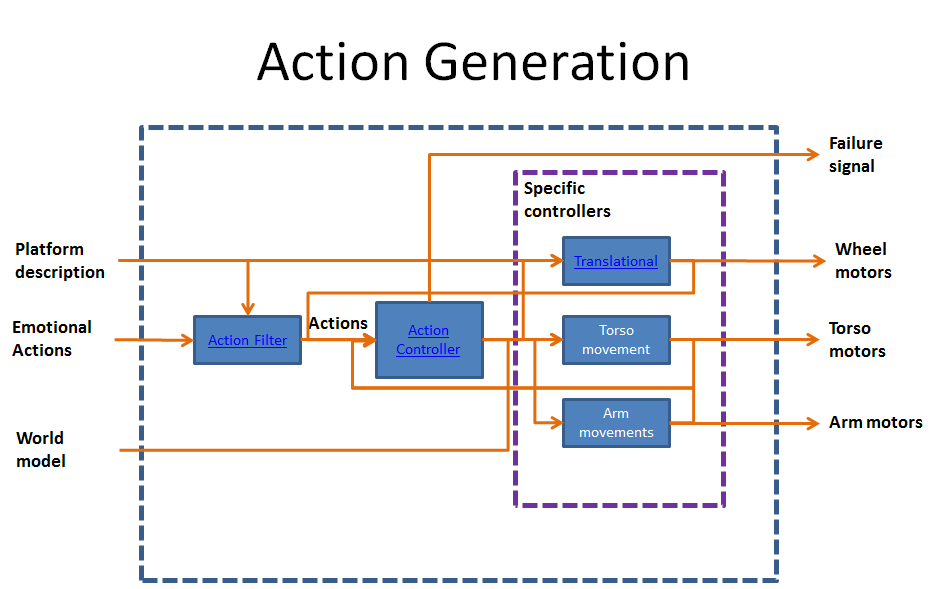
\includegraphics[width=1.0\textwidth]{./Images/Architecture/ActionGeneration.png} 
	\caption{Modules of the action generation}
	\label{fig:actionGeneration}
\end{figure}